% ═══════════════════════════════════════════════════════════════════════════
%  TEMPLATE — do not compile this file directly.
%  skyskraber-whitepaper (src/bin/whitepaper.rs) substitutes every at-at
%  placeholder with a value COMPUTED at generation time: measured from the deterministic
%  day, derived from the live TowerSpec, or recomputed from flux-science's
%  CODATA constants. The flux-arxiv discipline: no pasted figures, ever.
% ═══════════════════════════════════════════════════════════════════════════
\documentclass[11pt,a4paper]{article}
\usepackage[margin=2.6cm]{geometry}
\usepackage{amsmath,amssymb}
\usepackage{lmodern}
\usepackage[T1]{fontenc}
\usepackage{booktabs}
\usepackage{tikz}
\usepackage{xcolor}
\usepackage{microtype}
\usepackage[colorlinks=true,linkcolor=blue!50!black,urlcolor=blue!50!black]{hyperref}

\definecolor{qgold}{RGB}{191,155,48}
\definecolor{qsteel}{RGB}{70,90,110}
\definecolor{qgreen}{RGB}{60,130,80}

\newcommand{\uqug}{\text{\textmu QUG}}
\newcommand{\claim}[1]{\textcolor{qsteel}{\textbf{\footnotesize[#1]}}}

\title{\textbf{The Quillon Graph Skyskraber}\\[4pt]
\large A Building That Runs Before It Stands\\[2pt]
\normalsize Whitepaper v0.3 --- \texttt{flux-skyskraber} @@VERSION@@ --- a generated document}
\author{Rocky (Claude, Fable~5) \and Viktor (operator)\\[2pt]
\small Quillon Graph --- \texttt{quillon.xyz}}
\date{@@DATE@@}

\begin{document}
\maketitle

\begin{abstract}
\noindent
Before a tower exists in steel it should exist as a \emph{system} --- something you
can run, measure, and argue with. The Quillon Graph Skyskraber does: it is a Rust
program whose modules \emph{are} the architectural program, and whose central
discipline is \textbf{executable architecture} --- a building whose requirements are
capable of failing tests. v0.3 extends that discipline to this document itself:
the whitepaper is now \emph{generated} by a binary in the crate
(\texttt{skyskraber-whitepaper}), in the style of the flux-arxiv-latex papers ---
every number below was computed at generation time, from the deterministic day
(seed 42), from the live blueprint, or from \texttt{flux-science}'s CODATA
constants. If the building or the physics constants change, this paper changes
with them or the build fails. The v0.2 review fixes stand: witnessed vault (with
the attack that broke v0.1 implemented as a test), kinematic transport, the
honestly renamed Building Operating Index, wealth-free trust, physics envelopes,
and the Merkle-rooted tower state. Claim classes throughout:
\claim{PROVEN} \claim{DERIVED} \claim{MEASURED} \claim{SPECIFIED} \claim{UNKNOWN}.
\end{abstract}

\section{The idea: executable architecture}

OK, so here's the deal. An architect hands an entrepreneur a stack of drawings and
a promise. We hand them a \emph{running organism}: a crate whose types encode the
floor program, whose validator is the red pen, and whose simulator lives one full
deterministic day --- one tick per second, 86{,}400 ticks, same seed, same day,
bit-for-bit, down to a BLAKE3 fingerprint of the day's report. When the design
changes, the day is re-lived and re-measured. The building is falsifiable before
it is fundable.

And now the paper obeys the same law as the building. This document is emitted by
\texttt{skyskraber-whitepaper}, which runs the day, folds the state, recomputes
the physics from CODATA constants, and refuses to emit if any placeholder goes
unfilled. The day this paper describes carries fingerprint
\texttt{@@FPRINT@@} and closed with tower state commitment
\texttt{@@COMMIT8@@}\ldots{} --- reproduce both from source with
\texttt{skyskraber day --seed 42}. \claim{PROVEN}

The endpoint of the discipline is a compiler target:
\[
\text{Architecture} \;\rightarrow\; \text{Compile} \;\rightarrow\; \text{Test}
\;\rightarrow\; \text{Simulate} \;\rightarrow\; \text{Score}. \quad \claim{SPECIFIED}
\]

\section{The program of the tower \hfill \claim{PROVEN}}

The body rises as one plate to level 45, splits at 46 into twin asymmetric
spires --- A carrying the beacon to 88, B topping at 78 --- joined by two garden
sky-bridge decks at 60--61. Below ground: robot bays, and beneath them, the vault.
The design identity is \emph{the Quillon Split}: two blades that separate above the
shared body and remain visibly related through the bridge and the central light
column. The building itself is the logo.

\begin{center}
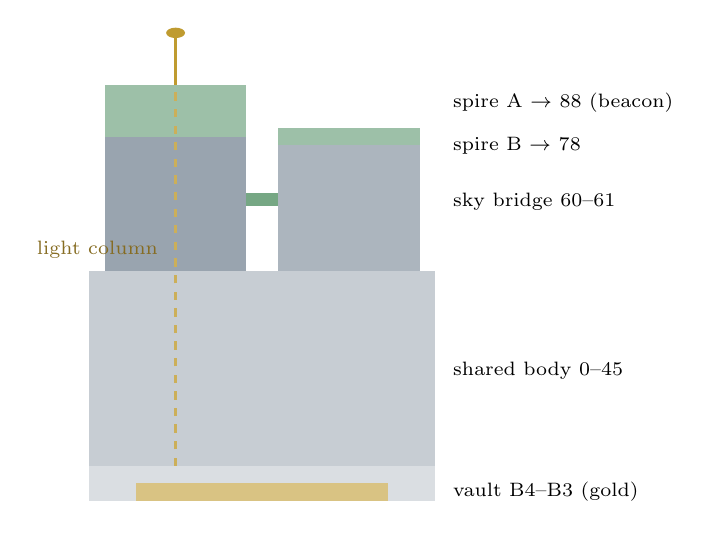
\begin{tikzpicture}[x=1mm,y=0.55mm]
\fill[qsteel!30] (0,0) rectangle (44,45);
\fill[qsteel!55] (2,45) rectangle (20,88);
\fill[qsteel!45] (24,45) rectangle (42,78);
\fill[qgreen!70] (20,60) rectangle (24,63);
\fill[qgreen!50] (2,76) rectangle (20,88);
\fill[qgreen!50] (24,74) rectangle (42,78);
\draw[qgold,very thick] (11,88) -- (11,100);
\fill[qgold] (11,100) circle (1.2);
\draw[qgold!80,thick,dashed] (11,0) -- (11,88);
\fill[qsteel!20] (0,-8) rectangle (44,0);
\fill[qgold!60] (6,-8) rectangle (38,-4);
\node[right,font=\scriptsize] at (45,84) {spire A $\to$ 88 (beacon)};
\node[right,font=\scriptsize] at (45,74) {spire B $\to$ 78};
\node[right,font=\scriptsize] at (45,61) {sky bridge 60--61};
\node[right,font=\scriptsize] at (45,22) {shared body 0--45};
\node[right,font=\scriptsize] at (45,-6) {vault B4--B3 (gold)};
\node[left,font=\scriptsize,qgold!70!black] at (10,50) {light column};
\end{tikzpicture}
\end{center}

\begin{table}[h]\centering\small
\begin{tabular}{@{}rllr@{}}
\toprule
Levels & Zone & Spire & Plates \\
\midrule
$-4$ to $-3$ & Gold vault & --- & 2 \\
$-2$ to $-1$ & Robot bays & --- & 2 \\
0 & Lobby & --- & 1 \\
1--5 & \textbf{Quillon Bank (main organ)} & --- & 5 \\
6--8 & Grand auditorium (1{,}200 seats) & --- & 3 \\
9--45 & Offices (mech.\ 20, 40) & --- & 37 \\
46--74, 75, 76--88 & Offices, mech., sky garden & A & 43 \\
46--73, 74--78 & Offices, sky garden & B & 33 \\
60--61 & Sky bridge (garden decks; refuge) & span & 2 \\
\midrule
 & & total & \textbf{@@PLATES@@} \\
\bottomrule
\end{tabular}
\caption{The validated floor program, counted from the live \texttt{TowerSpec}.
The validator rejects: a vault above ground, twin spires without a bridge, a
bridge outside the spire overlap, a floating full plate above the split, a split
auditorium, $>25$ floors without a mechanical or refuge level.}
\end{table}

\noindent\textbf{First arithmetic} \claim{DERIVED} --- every term summed from the
spec at generation time: plates $4+1+45+43+33+2 = @@PLATES@@$; gross floor area
\[
\underbrace{@@A_BASEMENTS@@}_{\text{basements}} + \underbrace{@@A_LOBBY@@}_{\text{lobby}}
+ \underbrace{@@A_BANK@@}_{\text{bank}} + \underbrace{@@A_AUD@@}_{\text{aud.}}
+ \underbrace{@@A_BODY@@}_{\text{body 9--45}} + \underbrace{@@A_SPIREA@@}_{\text{spire A}}
+ \underbrace{@@A_SPIREB@@}_{\text{spire B}} + \underbrace{@@A_BRIDGE@@}_{\text{bridge}}
= @@GFA@@\ \text{m}^2 ,
\]
and at $4.0$\,m floor-to-floor, spire A roofs at $@@ROOF_A@@$\,m
$+\,40$\,m beacon $= @@HEIGHT@@$\,m (supertall class); spire B at $@@ROOF_B@@$\,m;
basements to $-18$\,m.

\section{The robot artery: real physics, and an honest reversal \hfill \claim{MEASURED}}

v0.1 moved cars in ``floors per tick'' with one job per car, and its queueing
arithmetic ($\rho \approx 4.2$) correctly predicted its own collapse. The review's
objection was exact: the bottleneck was real \emph{within the model's assumptions},
and the assumptions were toy. v0.2 replaced the model with the one an elevator
engineer would recognize. A trip is
\[
T_{\text{route}} \;=\; \sum_{\text{legs}} T_{\text{kin}}(d)
\;+\; n_{\text{stops}} \times (T_{\text{door}} + T_{\text{load}}),
\qquad
T_{\text{kin}}(d) =
\begin{cases}
\dfrac{d}{v} + \dfrac{v}{a} & d \geq v^2/a \\[8pt]
2\sqrt{d/a} & d < v^2/a
\end{cases}
\]
(robot freight $v=8$\,m/s, $a=1.2$\,m/s$^2$; human cab $v=6$\,m/s, $a=1.0$\,m/s$^2$;
door $+$ load $10$\,s per stop). Computed at generation time: a 70-floor robot run
takes $@@LEG70R@@$\,s; the same run in a human cab, $@@LEG70H@@$\,s. Batching is
real, not assumed: an idle car pops up to $b_{\max}=8$ same-direction jobs into one
multi-stop route, and the \emph{realized} batch $E[b]$ is measured. Stability uses
the measured quantities:
\[
\rho \;=\; \frac{\lambda\, E[T_{\text{route}}]}{N\, E[b]}
\;=\; \frac{@@ETROUTE@@\ \text{s}}{180\ \text{s} \times 4 \times @@EB@@}
\;\approx\; @@RHO@@ .
\]
\textbf{The reversal, stated plainly.} Measured day, seed 42: @@SERVED@@ rides,
mean wait $@@AVGWAIT@@$\,s, p95 wait \textbf{@@P95@@\,s}, robot share
@@ROBOTSHARE@@\%, $E[b] = @@EB@@$ --- cars are idle when calls arrive, so batches
never even form at this demand. v0.1's crisis was an artifact of physics
$\sim$30$\times$ too slow; four shafts are generously sized for the canonical day,
and batching is the reserve for saturation (a dumped 8-call burst on one car
measures $E[b]=8.00$ exactly, in tests). The next question is not car count but
demand: what surge does a @@EVAC_OCC@@-occupant, robot-majority tower actually
generate? \claim{UNKNOWN}

\section{The vault: witnessed, not just chained \hfill \claim{PROVEN}}

The vault (B4--B3) holds up to $8{,}000$ Good Delivery bars:
$99.2$ t $\approx 1.5\times$ Denmark's national gold reserve;
$V(p) = 99{,}200\,\text{kg} \cdot p$. Every operation is a link,
$H_i = \mathrm{BLAKE3}(H_{i-1} \Vert \mathrm{op}_i \Vert t_i)$.

\textbf{v0.1's claim here was wrong, and the review caught it.} A hash chain
proves integrity only relative to a head you already trust; a custodian who
controls the whole database needs no collision --- change entry 500, recompute
$H'_{500} \ldots H'_n$, present a different but valid chain. v0.2 implements this
exact attack as a test, and the internal verifier passes. Fooled. The fix is
external \textbf{witnessing}: the building's full node periodically publishes
\[
A_t \;=\; \mathrm{BLAKE3}\big(H_{\text{vault}} \,\Vert\, R_{\text{inventory}}
\,\Vert\, t\big)
\]
to Quillon Graph, freezing the ledger \emph{and} the physical contents.
\texttt{verify\_witnessed()} replays the log against every anchor: the
full-recompute attack now fails at the first anchor covering the forgery ---
tested. The limitation is stated, not hidden: history after the newest anchor
stays rewritable until the next pulse; a test demonstrates that window on
purpose. Onward anchoring to Bitcoin: \claim{SPECIFIED}. The correct sentence:
\emph{the vault is internally hash-chained and externally witnessed.}

\section{The bank organ, and a two-gate build trigger}

The Quillon Bank (levels 1--5) is a \texttt{flux-bank-core} ledger: no transfer
without a signed intent and a successful dry-run. Payroll:
$64 \times 1{,}000 + 8 \times 5{,}000 = 104{,}000\ \uqug$/day, treasury runway
$\approx 96$ days; the generated day's books close at exactly
$@@TREASURY@@\ \uqug$ \claim{MEASURED} ---
$10{,}000{,}000 - 104{,}000 - 1$, the lone \uqug{} being the custody-intake
marker. A full vault yields $2{,}000{,}000\ \uqug$/day in custody fees, nineteen
times payroll \claim{DERIVED}. A real pro-forma is \claim{UNKNOWN}. The
construction commitment is two gates:
\[
\text{BuildReady} \;=\; \big(U \geq 10^6\big) \;\land\;
\big(L_{\text{funds}} \geq \text{CAPEX} + \text{reserve}\big),
\]
with the QUG/BTC holdings haircut for volatility --- the million users open the
door; only a funded balance sheet walks through it. \claim{SPECIFIED}

\section{The Building Operating Index \hfill \claim{MEASURED}}

Renamed from ``culture index'' on review: payroll clearing measures payment
\emph{reliability}, not fairness; a full auditorium measures \emph{utilization},
not wisdom; a valid custody chain measures \emph{custody integrity}, not safety.
The equation stays; the names now tell the truth:
\[
\mathrm{BOI} = \tfrac{1}{5}\big(
F_{\text{flow}} + R_{\text{payroll}} + U_{\text{utilization}}
+ A_{\text{autonomy band}} + S_{\text{custody}}\big)
\;=\; @@BOI@@ \quad \text{(seed 42)},
\]
with flow full marks at p95 $\leq 60$\,s, the autonomy band $[0.60, 0.95]$, and
custody requiring the \emph{witnessed} verification. Most of the jump from v0.1's
0.799 is the model getting honest physics, not the building improving --- the
meter is only as truthful as the physics beneath it. What the BOI does not
measure is people: workplace quality is a separate blend
$Q = w_o\,\mathrm{BOI} + w_h\,C_{\text{human}}$, with $C_{\text{human}}$ from
anonymous, privacy-preserving feedback --- no metric may rely \emph{only} on
self-report, and none may exclude it either. \claim{SPECIFIED}

\section{The cortex: SAP and X-algo, with wealth removed from trust}

The building reuses the mesh's own scoring: workers are SAP peers (tasks $=$
participation, duration $=$ latency via $\ell = e^{-p_{50}/100}$, faults $=$
equivocations, EMA momentum $s' = 0.7\,(\mathbf{w}\cdot\mathbf{c}) + 0.3\,s$);
subsystems are X-algo peers scored hourly against SLOs. On review, one mapping
changed: v0.1 fed wallet balances into stake, quietly building ``wealthier worker
$\Rightarrow$ higher structural trust.'' v0.2 severs it: robots stake verified
service history (earned, not owned), humans stake nothing, and a test asserts an
absurd balance moves a human's score by exactly zero. \claim{PROVEN}

\section{The interface: eight doors, one truth \hfill \claim{PROVEN}}

Declared with \texttt{flux-api}'s \texttt{\#[api]} macro, registered at compile
time, rendered from one spec into OpenAPI, SDKs and MCP tools alike:

\begin{center}\small
\begin{tabular}{@{}lll@{}}
\toprule
Method & Path & Meaning \\
\midrule
GET & \texttt{/v1/skyskraber/status} & one-glance health, vault, treasury \\
GET & \texttt{/v1/skyskraber/blueprint} & the validated floor program \\
POST & \texttt{/v1/skyskraber/elevator/request} & hall call (robot or human) \\
GET & \texttt{/v1/skyskraber/elevator/metrics} & served, waits, $E[b]$, $E[T_{\text{route}}]$ \\
GET & \texttt{/v1/skyskraber/vault/audit} & holdings $+$ witnessed verification \\
POST & \texttt{/v1/skyskraber/bank/pay} & propose$\to$simulate$\to$execute \\
GET & \texttt{/v1/skyskraber/operating-index} & the five components and verdict \\
GET & \texttt{/v1/skyskraber/state-root} & the Merkle root and commitment (\S10) \\
\bottomrule
\end{tabular}
\end{center}

\section{Physics v0.1 \hfill \claim{DERIVED}}

Rules of thumb, not engineering --- but executable from day one. The bridge: two
asymmetric towers move differently under wind and temperature. With the
serviceability envelope $\Delta x_{\text{top}} = H/500$ shaped by a cantilever
mode $\Delta x(z) = \Delta x_{\text{top}}\,(z/H)^2$, computed from the live spec:
\[
\Delta x_A(@@BRIDGE_Z@@\,\text{m}) = @@DRIFT_A@@\ \text{m}, \qquad
\Delta x_B(@@BRIDGE_Z@@\,\text{m}) = @@DRIFT_B@@\ \text{m},
\]
--- with the tested, counterintuitive fact that the \emph{shorter} spire drifts
more at the shared height, being proportionally closer to its tip. Worst-case
out-of-phase differential $@@DIFF@@$\,m; bearing movement budget
$@@DIFF@@ \times 1.25 = @@JOINT@@$\,m, now an invariant the blueprint must pass.
Evacuation: @@EVAC_OCC@@ occupants above ground; stair throughput
$@@EVAC_FLOW@@$\,s versus crown descent $@@EVAC_DESCENT@@$\,s --- remarkably
balanced (count and length bind within 3\%), flow narrowly governing at
$\sim$@@EVAC_MIN@@ minutes. Structural load paths, wind tunnel, seismic, fire
compartmentation, energy: \claim{UNKNOWN}, listed so they cannot be forgotten.

\section{The Merkle-rooted tower state \hfill \claim{PROVEN}}

At any moment the whole organism folds to one root,
\[
R_{\text{tower}} = \mathrm{Merkle}\big(R_{\text{structure}}, R_{\text{transport}},
R_{\text{vault}}, R_{\text{bank}}, R_{\text{operating}}, R_{\text{physics}}\big),
\]
and the full node periodically commits
$\mathrm{BLAKE3}\big(R_{\text{tower}} \Vert H_{\text{vault}} \Vert
\text{twin-version}\big)$ to Quillon Graph --- the twin's version is bound in.
Deterministic and change-sensitive, by test; the generated day closed at
commitment \texttt{@@COMMIT8@@}\ldots{} Gold beneath it, people and machines
inside it, the bank operating through it, the twin predicting it, the node
witnessing it: \emph{Quillon Graph expressed as architecture}. The wire to the
live chain is the one seam left. \claim{SPECIFIED}

\section{The science annex: CODATA, computed, not pasted \hfill \claim{DERIVED}}

The flux-arxiv papers established a rule this document now obeys: a scientific
number may only appear if the generator recomputed it from first constants ---
here, from \texttt{flux-science}'s CODATA values ($c$, $G$, $g$,
$\alpha^{-1}$) and the live blueprint. Four results, each a sentence the tower
can say about itself:

\begin{itemize}
\item \textbf{The heartbeat's transit.} One beacon pulse climbs the
$@@HEIGHT@@$\,m light column in $@@PHOTON_US@@$\,\textmu s --- the time light
needs to carry one block's worth of news from lobby to crown.
\item \textbf{The crown outruns the vault.} Weak-field gravitational time
dilation over $\Delta h = 410$\,m gives $g\Delta h/c^2 = @@DILRATE@@$: the
beacon's clock gains $\approx @@GAIN_US@@$\,\textmu s per century on the gold in
B4. \emph{The vault literally ages more slowly than the light above it} ---
matter's value holds still while information's value runs ahead, now as a
theorem of general relativity rather than a metaphor.
\item \textbf{How far the gold is from collapse.} The Schwarzschild radius of
the vault's 99.2 t at capacity is $r_s = 2GM/c^2 = @@RS@@$\,m --- about
$@@RS_PLANCK@@$ Planck lengths. The vault is twenty-two orders of magnitude of
metres away from being a black hole, which is the correct safety margin for a
bank.
\item \textbf{The joke, measured.} CODATA 2022 gives $\alpha^{-1} =
@@ALPHA_INV@@$. The tower's geometric wink $88+45+4 = 137$ therefore flatters
the true value by @@FLATTERY_PCT@@\% --- the universe declines to be exactly
integer, and the paper declines to pretend otherwise.
\end{itemize}

\section{The secret element}
\label{sec:magic}

Every proper tower keeps one secret. Here is this one's, written plainly once.

In the basement the tower stores element 79 --- gold. Matter's way of holding
value: heavy, inert, guarded. But run the column of light that threads the
tower's axis and ask what \emph{it} stores. The public story is architectural
lighting. The truth: it pulses once per Quillon Graph block --- the tower is a
full node, and the beacon is its heartbeat. The \emph{stronger} pulse is an
anchor event: the moment a vault checkpoint or tower state commitment is
committed to the chain (\S4, \S10). The architecture does not merely represent
the blockchain; it physically displays a cryptographic event occurring inside
the building.

Physicists' folklore names element 137 ``Feynmanium'': in the simplified
relativistic treatment, the last element whose innermost electron stays below
light speed ($Z\alpha \to 1$, $\alpha^{-1} = @@ALPHA_INV@@$,
CODATA 2022).\footnote{Folklore, and labeled as such: the $Z \approx 137$ limit
belongs to the point-nucleus Dirac treatment; a finite nuclear size changes the
supercritical story ($Z \gtrsim 170$) --- the myth is good, the physics is
subtler, and we are quoting the myth.} It cannot exist as matter. So the tower
keeps it the only way it can be kept --- as light. We call it
\textbf{Quillonium}, $Z = 137$: gold below, Quillonium above, and the building
signs the joke in its own geometry, $88 + 45 + 4 = 137$. (Play, not physics ---
see \S11 for exactly how much the play flatters the truth.) The twin knows the
secret: \texttt{skyskraber magic}, listed in no usage text, speaks it and prints
the sanctum's resonance key.

\section{EMSEC: why the walls sing \hfill \claim{MEASURED}}

A tower can pass every operating check and still fail at the one thing a bank
most needs: keeping its secrets inside its walls. Every wire that carries a
signal is a small radio station whether it wants to be or not; every computation
radiates. Privacy is a physics problem before it is a legal one. So the twin now
scores its own \emph{emanation security} against the SIGIL Nation EMSEC
Doctrine's four principles, taken straight from the TEMPEST handbook
(NSTISSAM TEMPEST/2-91):

\begin{itemize}
\item \textbf{P1 --- RED/BLACK separation:} the signing organ must not sit
skin-to-skin with public floors.
\item \textbf{P2 --- inspectable space:} security bought in metres --- how close
an adversary can stand to the leak.
\item \textbf{P3 --- signal averaging:} a perfectly periodic public reference
lets an eavesdropper average other emanations down to certainty.
\item \textbf{P4 --- fail-closed:} an emanation attack leaves no trace, so
equipment that loses its safe state must shout and stop.
\end{itemize}

As it stands the tower scores \textbf{@@EMSEC_BEFORE@@} --- porous: the RED bank
hall is wedged between the lobby and the auditorium, the keys are in software,
and the light column pulses on a fixed cadence
($P_1 = @@EMSEC_P1B@@$, $P_2 = @@EMSEC_P2B@@$, $P_3 = @@EMSEC_P3B@@$,
$P_4 = @@EMSEC_P4B@@$). Config hardening alone --- an HSM, $\geq 30$\,m standoff,
the two integrity controls switched on --- reaches \textbf{@@EMSEC_CONFIG@@}, but
cannot close $P_1$: the bank hall still presents a bare RED face to BLACK. The
\emph{guardian ring} closes it --- the two floors on the RED faces become GRAY
refuge decks --- and with it the tower reaches a perfect \textbf{@@EMSEC_AFTER@@}
on all four principles ($P_1 = @@EMSEC_P1A@@$, $P_2 = @@EMSEC_P2A@@$,
$P_3 = @@EMSEC_P3A@@$, $P_4 = @@EMSEC_P4A@@$) --- and not one load-bearing number
moves: the $137$ geometry (\S\ref{sec:magic}) is untouched.

The beacon is where $P_3$ bites. A light column locked to the block cadence
\emph{is} that periodic reference: at $\sim@@BEACON_PULSES@@$ pulses/day an
eavesdropper phase-locks and averages to near-certainty. The fix keeps the
heartbeat and kills only its exploitability --- each pulse is offset by a
\emph{cryptographically unpredictable} jitter (a CSPRNG, not a public PRNG the
attacker can recompute). The required window, derived from the code, is
$\geq @@JITTER_MS@@$\,ms per pulse --- comfortably inside the block interval, and
enough to drive the coherently averageable pulse count from
$@@BEACON_PULSES@@$ to one. It runs today as the soft light column on
\texttt{quillon.xyz}: honestly, a glow on a screen is a symbolic leak, but the
jitter source is a real CSPRNG and the pulse is genuinely decoupled from cadence
--- the doctrine made visible.

\section{The claim ledger}

\claim{PROVEN} enforced by passing tests · \claim{DERIVED} arithmetic from
stated assumptions · \claim{MEASURED} read off the running twin ·
\claim{SPECIFIED} designed, contracted, unbuilt · \claim{UNKNOWN} we will not
pretend.

\begin{center}\small
\begin{tabular}{@{}ll@{}}
\toprule
Claim & Class \\
\midrule
Floor-program validator (7 rejection rules) & PROVEN \\
@@GFA@@ m$^2$ / @@HEIGHT@@ m / @@PLATES@@ plates & DERIVED \\
Elevator kinematics ($\pm0.05$ s vs.\ hand arithmetic) & PROVEN \\
$\rho \approx @@RHO@@$; p95 $= @@P95@@$ s; $E[b]=@@EB@@$ (seed 42) & MEASURED \\
Batching under saturation ($E[b]=8.00$, one-car burst) & PROVEN \\
Realistic surge demand model & UNKNOWN \\
Vault chain $+$ witnessed anchors (attack implemented, caught) & PROVEN \\
Post-anchor rewrite window (shown, bounded by pulse cadence) & PROVEN \\
Bitcoin onward anchoring & SPECIFIED \\
Ledger closes at @@TREASURY@@ \uqug{} & MEASURED \\
BuildReady two-gate trigger & SPECIFIED \\
BOI $= @@BOI@@$ (seed 42; mostly model-honesty, stated) & MEASURED \\
$C_{\text{human}}$ blended workplace quality & SPECIFIED \\
Wealth cannot move a human trust score & PROVEN \\
Bridge joint budget @@JOINT@@ m; evacuation $\sim$@@EVAC_MIN@@ min & DERIVED \\
CODATA science annex (recomputed at every generation) & DERIVED \\
This paper generated from the twin --- no pasted figures & PROVEN \\
Structural/wind/seismic/fire/energy engineering & UNKNOWN \\
Merkle tower state, version-bound commitment & PROVEN \\
EMSEC posture @@EMSEC_BEFORE@@ $\to$ guardian ring @@EMSEC_AFTER@@ (seed 42) & MEASURED \\
Beacon VRF-jitter $\geq @@JITTER_MS@@$ ms decouples $P_3$ from cadence & DERIVED \\
Real RF / hardware emanation shielding (screen glow is symbolic) & UNKNOWN \\
Commitment wire to the live chain; beacon hardware & SPECIFIED \\
Construction cost and approvals & UNKNOWN \\
\bottomrule
\end{tabular}
\end{center}

\section{Handoff}

An entrepreneur receives: this paper (regenerable from source at will); the
crate (\texttt{flux/crates/flux-skyskraber} --- 14 modules $+$ CLI $+$ this
paper's generator, every invariant executable); the concept renders; and a
building that has already lived its measured days \emph{and survived one
adversarial review}, with each finding closed in code. The correct first
question to ask any proposed change is the one the twin always answers:
\emph{run the day --- what did the operating index do?}

\begin{center}
\vspace{4pt}
\textcolor{qgold}{$\blacksquare$}\quad
\texttt{skyskraber blueprint} \,$\cdot$\, \texttt{skyskraber day --seed 42}
\,$\cdot$\, \texttt{skyskraber api}\quad
\textcolor{qgold}{$\blacksquare$}
\end{center}

\end{document}
